
\newpage
\appendix

\section{附录}

\subsection{数学符号说明}
\begin{table}[h]
\centering
\caption{数学符号说明}
\label{tab:symbols}  % 添加这一行
\begin{tabular}{cl}
\hline
\textbf{符号} & \textbf{含义} \\
\hline
\multicolumn{2}{c}{\textbf{基本变量}} \\
\hline
$\mathcal{A}$ & 描述硬币A投掷结果的随机变量\\
$\mathbb{A}$ & 随机变量$\mathcal{A}$的取值集合,本例中为$\{0,1\}$  \\
$o_i$ & 第$i$次观测结果,$o_i \in \{0,1\}$ \\
$n$ & 观测次数 \\
$\hat{o}$ & 样本中正面结果的比例,$\hat{o} = \frac{1}{n}\sum_{i=1}^n o_i$ \\
\hline
\multicolumn{2}{c}{\textbf{参数相关}} \\
\hline
$\pi = (p_A, p_B, p_C)$ & 三个硬币投出正面的概率参数向量 \\
$\pi^{(t)}$ & EM算法第$t$次迭代的参数估计 \\
$\xi$ & 边缘概率,$\xi = p_A p_B + (1-p_A) p_C$ \\
$r_1, r_0$ & 观测到正面/反面时硬币A被选中的后验概率 \\
\hline
\multicolumn{2}{c}{\textbf{函数与分布}} \\
\hline
$L(\pi)$ & 对数似然函数 \\
$q_t^i(a)$ & 第$t$次迭代时观测$o_i$下隐变量$\mathcal{A}=a$的后验概率 \\
$Q(\pi|\pi^{(t)})$ & EM算法中的Q函数(期望完整数据对数似然) \\
$p(o_i, \mathcal{A}=a; \pi)$ & 观测值和隐变量的联合概率 \\
$\mathcal{N}(\mu, \sigma^2)$ & 均值为$\mu$、方差为$\sigma^2$的正态分布 \\
\hline
\multicolumn{2}{c}{\textbf{算法相关}} \\
\hline
$\argmax$ & 使目标函数达到最大值的参数 \\
$\mathcal{L}(q,\theta)$ & 证据下界(ELBO) \\
$\theta$ & 一般参数记号 \\
$T$ & EM算法的迭代次数 \\
\hline
\end{tabular}
\end{table}


\subsection{附加实验}
本附加实验旨在从参数空间的角度直观展示 EM 算法对不同初始值的收敛行为。具体步骤如下:

\begin{enumerate}
  \item 在 $[0.05,0.95]^3$ 范围内均匀采样若干组初始参数 $(p_A,p_B,p_C)$;
  \item 对每组初始值仅执行两步 EM 迭代,记录迭代结束后的收敛点 $\theta_{\rm final}=(p_A,p_B,p_C)$;
  \item 利用径向基函数(RBF)插值,在 $(p_A,p_B)$ 网格上对所有收敛点拟合出平滑曲面 $p_C=f(p_A,p_B)$,从而得到左图所示的“收敛结果曲面”;
  \item 计算每个收敛点在观测数据下的平均对数似然值,并在真参数对应的对数似然水准上应用 marching\_cubes 算法提取三维等值面,得到右图所示的“对数似然等值面”。
\end{enumerate}
\begin{figure}[H]
  \centering
  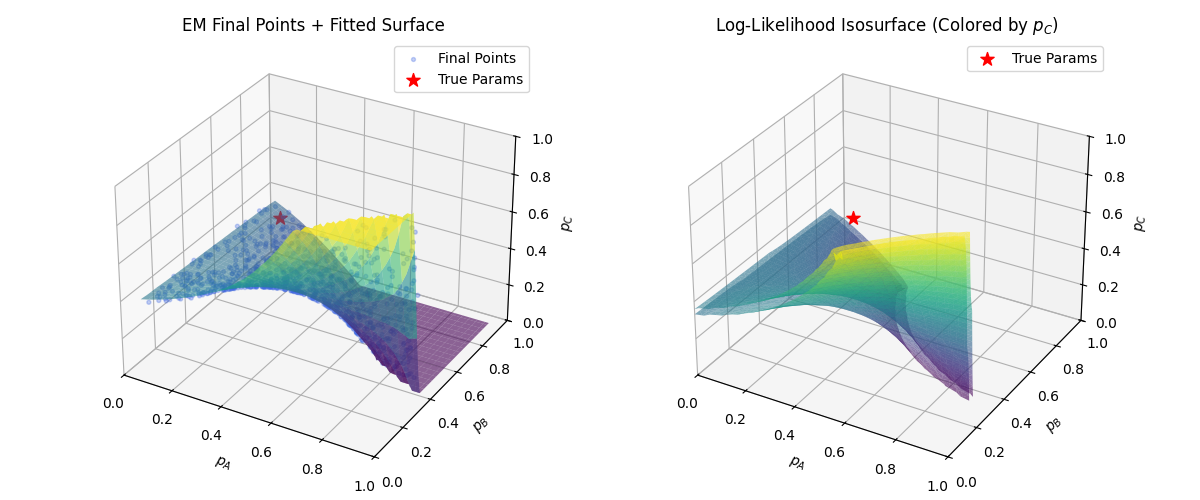
\includegraphics[width=0.75\textwidth]{../images/sur.png}
  \caption{左图为不同初始点导致的不同收敛结果组成的收敛结果曲面,右图为收敛结果对应的似然值导出的对数似然等值面}
  \label{fig:sur}
\end{figure}

\subsection{思维导图}
\begin{figure}[H]
  \centering
  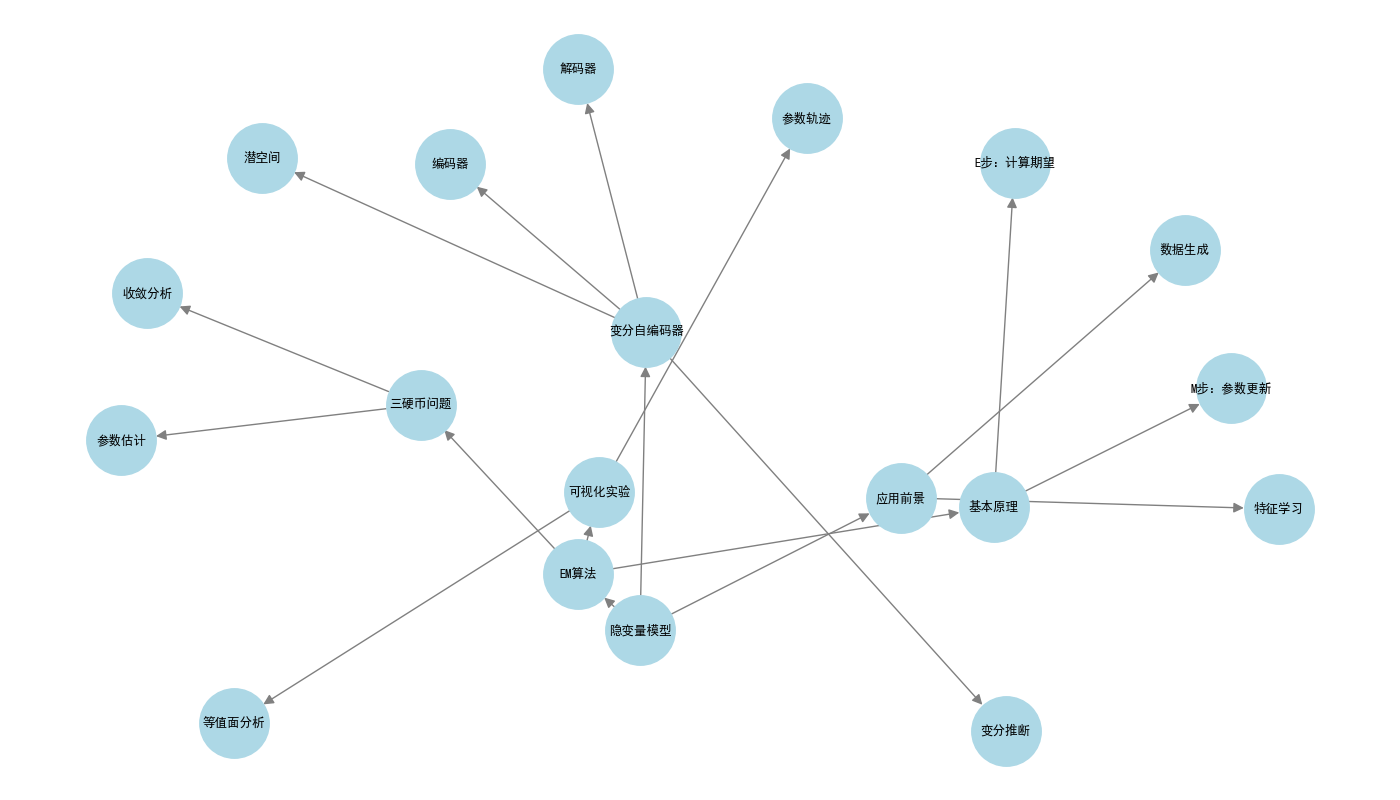
\includegraphics[width=0.75\textwidth]{../images/mind.png}
  \caption{思维导图}
  \label{fig:mind}
\end{figure}